\documentclass[10pt,a4paper]{article}
\usepackage[utf8]{inputenc}
\usepackage[english]{babel}
\usepackage{url}
\usepackage{hyperref}
\usepackage{amsmath}
\usepackage{amsfonts}
\usepackage{amssymb}
\usepackage{graphicx}
\usepackage{float}
\usepackage{lipsum}
\usepackage{multicol}
\usepackage{xcolor}
\newcommand{\celda}[1]{
	\begin{minipage}{2.5cm}
		\vspace{5mm}
		#1
		\vspace{5mm}
	\end{minipage}
}
\definecolor{azul}{rgb}{0.0, 0.53, 0.74}
\usepackage[left=2.00cm, right=2.00cm, top=2.00cm, bottom=2.00cm]{geometry}


\begin{document}

	\vspace{7.5mm}
	
	\begin{center}
		{\Large \textbf{A Hybrid Quantum-Classical Computational
Study of Energetic and Conformational Differences in Amyloid-$\beta$ variants}}\\
		\vspace{2mm}
		{\large Kushal Patil$^{1}$}\\
		\vspace{7.5mm}
		$^1$\textit{Student, Lincoln Sudbury Regional High School, 390 Lincoln Road, Sudbury, MA 01776, USA} \\
	\end{center}

	\begin{center}
		\textcolor{azul}{\rule{150mm}{0.5mm}}
	\end{center}		

	\begin{abstract}
        %\textit{\textbf{To Dr. Shao: What I understand is needed to improve this paper is increasing the sample size, increasing the statistical rigor, and proving the VQE's detection of electronic signatures in aggregation-prone structures using Secondary Structure graphs and Radius of gyration graphs from MD. I also should incorporate more exp. data to further validate my claims...}}\\
        
		The objective for this project is to apply a hybrid quantum-classical approach with all-atom MD and Variational Quantum Eigensolver (VQE) to analyze electronic level differences between Amyloid-$\beta$ variants that influence mutation-driven protein aggregation in Alzheimer's Disease. Alzheimer’s disease, the most common form of dementia, affects seven million people in the US alone. A defining molecular hallmark of the disease is the accumulation of extracellular plaques composed of beta-amyloid (A$\beta$). In particular, the Arctic variant of A$\beta$ exhibits accelerated aggregation compared to wild-type peptides. Computational approaches such as all-atom molecular dynamics (MD) remain limited in their ability to look into the quantum-level electronic properties that underpin the aggregation propensity. Molecular dynamics simulations sampled wild-type and Arctic amyloid-$\beta$ structures. Stable LVFFA fragments were extracted, capped, and analyzed with DFT. Active-space Hamiltonians were mapped to qubits for Variational Quantum Eigensolver simulations. Electronic energy differences between mutant and wild-type variants were calculated, then validated by ORCA B3LYP. This workflow links long-timescale MD sampling to quantum electronic structure analysis, targeting mutation-induced aggregation effects in neurodegenerative disease. The results were ambiguous and leaned toward a more stable Arctic variant compared to the wild-type's structure. The Arctic variant displayed more compact $\beta$-sheet-rich conformations in MD, consistent with aggressive protein aggregation. Quantum-calculated energy gaps between wild-type and mutant fragments correlated with HOMO-LUMO shifts, suggesting electronic-level mutation effects. DFT (B3LYP/ORCA) benchmarks confirmed quantum simulations’ accuracy. These results demonstrate that quantum electronic descriptors capture the mutation’s impact and support the computational approach’s relevance for studying neurodegeneration. VQE simulations on these reduced Hamiltonians reveal an electronic stabilization in the Arctic variant compared to the wild-type protein. This suggests a direct quantum-level contribution to its propensity for aggregation. Our results demonstrate a transferable workflow for probing biomolecular electronic structure on near-term quantum devices, bridging molecular biophysics and quantum computation for larger systems.
\vspace{2mm}

\underline{\textbf{Keywords:}} \hspace{1mm} \textit{VQE, Amyloid Beta, Wild-type, Arctic}
	\end{abstract}

	\begin{center}
		\textcolor{azul}{\rule{150mm}{0.5mm}}
	\end{center}		

	\vspace{5mm}
	
	\begin{multicols}{2}
		\section{Introduction}
		Alzheimer’s disease, the most common form of dementia, affects millions of people in the United States and represents a critical biomedical and social challenge. A defining molecular hallmark of the disease is the accumulation of extracellular plaques composed of beta-amyloid (A$\beta$) peptides. In particular, the Arctic variant of A$\beta$ with the E22G mutation is associated with hereditary Alzheimer’s that exhibits accelerated aggregation compared to wild-type peptides, making it an important target for study. Computational approaches such as all-atom molecular dynamics (MD) have provided invaluable insights into A$\beta$ structure and dynamics, yet remain limited in their ability to look into the quantum-level electronic properties that underpin the aggregation propensity. Here, I propose a combined classical–quantum workflow that integrates MD simulations with quantum algorithms, a Variational Quantum Eigensolver (VQE\cite{peruzzo2014}), to examine electronic structure features of A$\beta$ peptide fragments, specifically the hydrophobic LVFFA core(Figure 1). This hybrid approach aims to accelerate current simulation workflows while offering deeper mechanistic insights and paving the way for broader applications in the study of protein misfolding and other complex biophysical systems.
        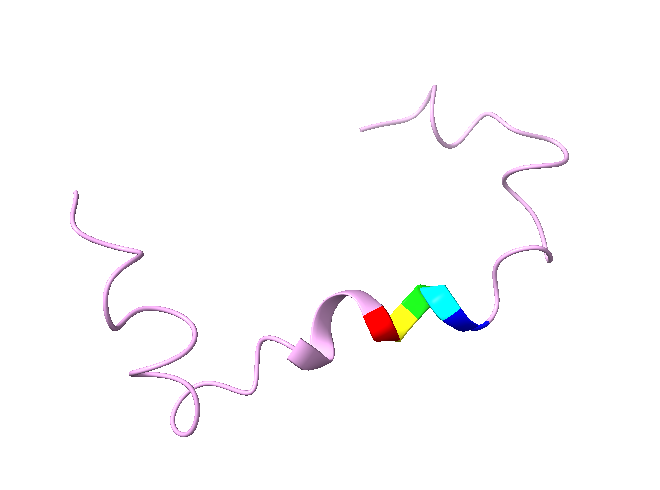
\includegraphics[width=1\linewidth]{LVFFA.png}
        \caption\textbf{Figure 1: }{Wild Type Amyloid beta with LVFFA core highlighted}


			
		\section{Procedure}
	\end{multicols}
	

	\begin{multicols}{2}
        The methodology involves a multi-faceted approach that bridges all-atom molecular dynamics with quantum algorithms (Figure 2). This reduces the runtime and allows for deeper insights than classical methods.\\
        
        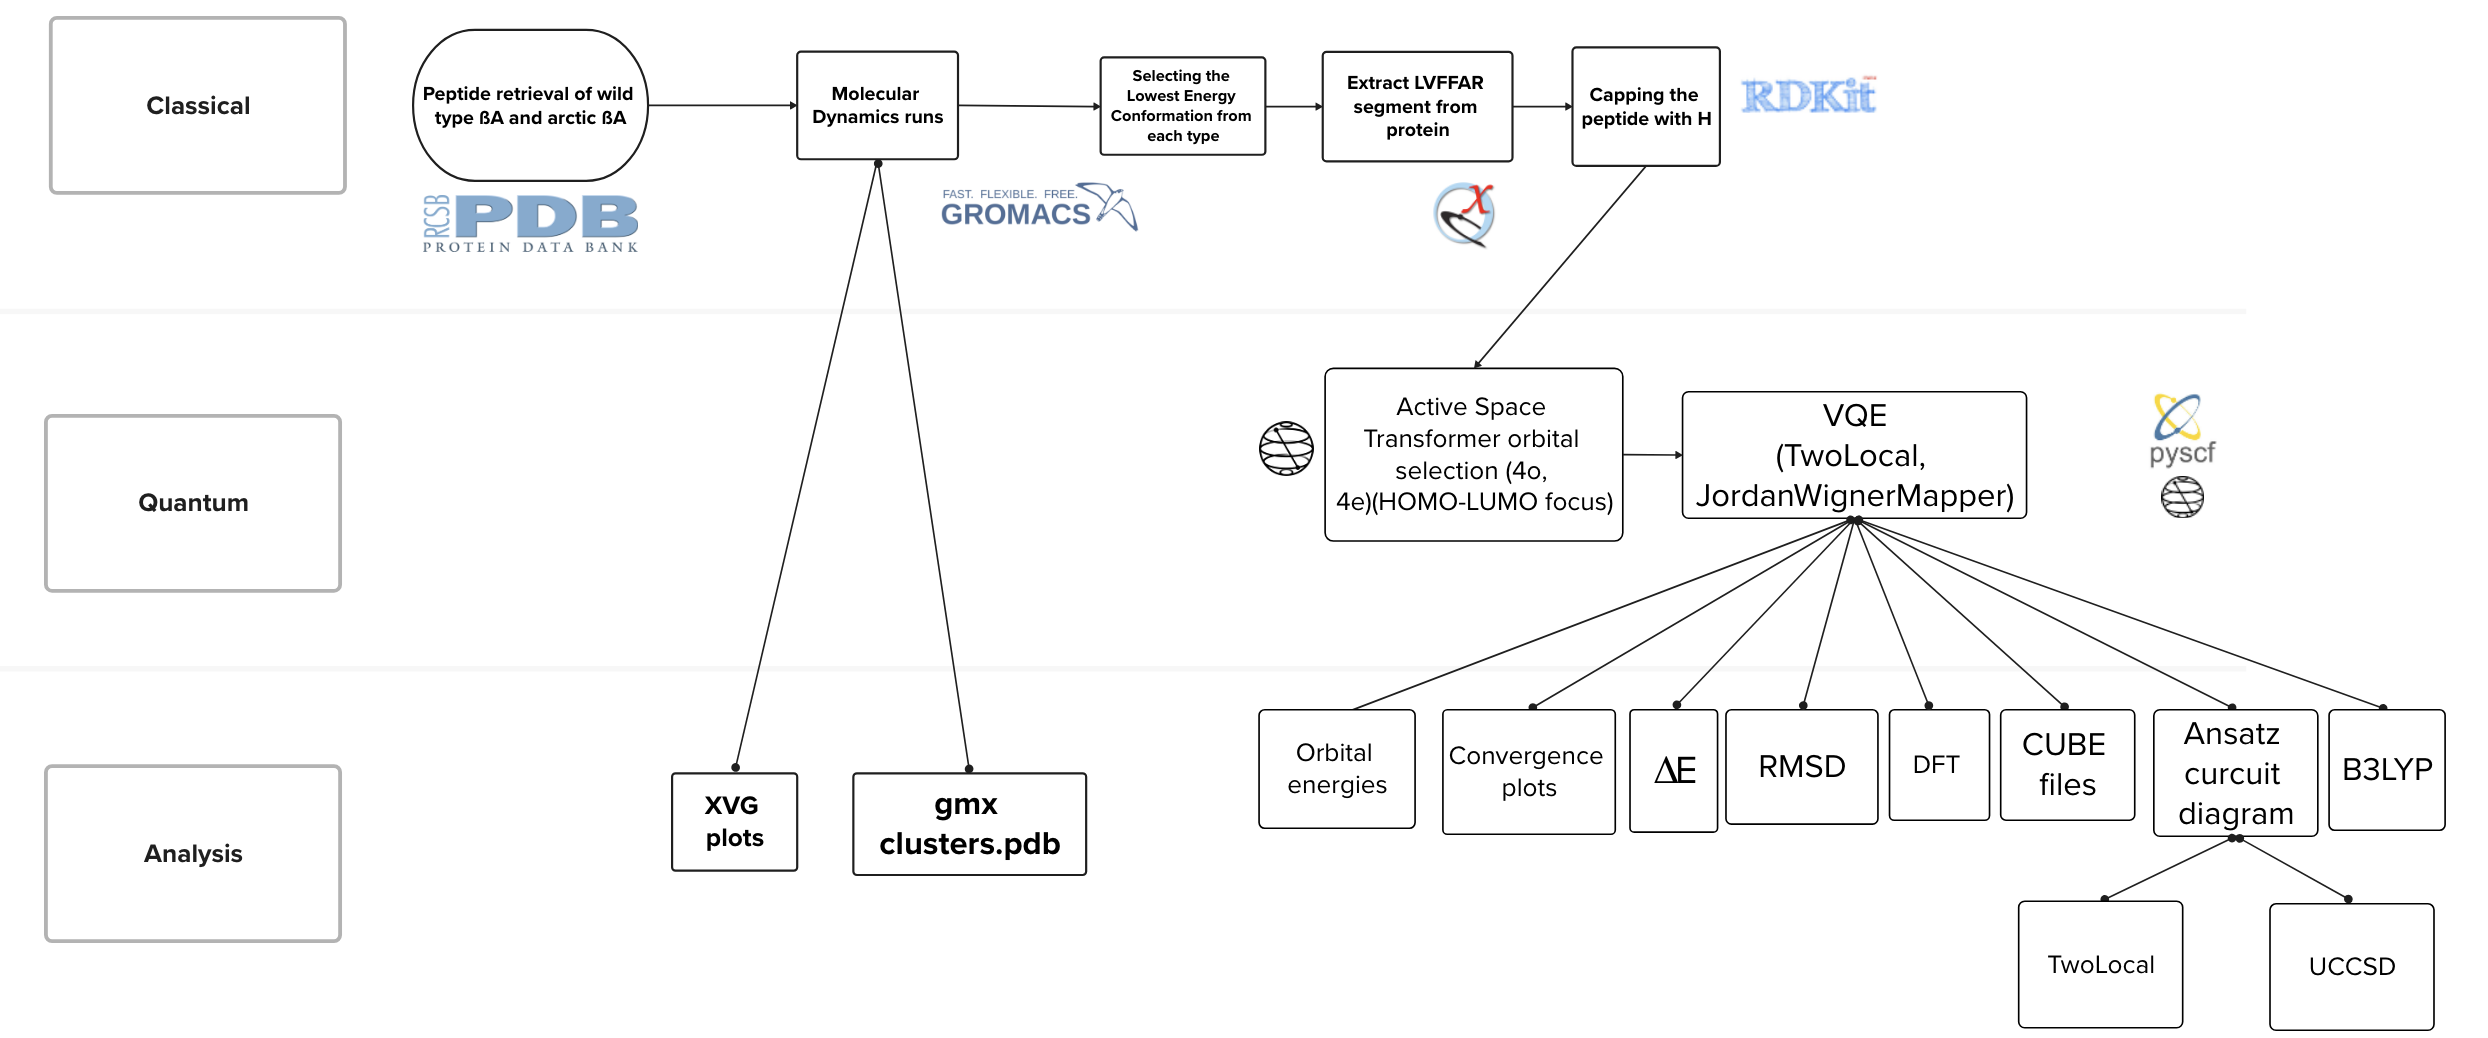
\includegraphics[width=1\linewidth]{Schematic.png}
 \caption \textbf{Figure 2: }{Schematic depicting the methodology and flow from MD of all-atoms to Quantum runs, while also depicting the material analyzed} 
        \subsection{All Atom MD}
        All-atom simulations were performed with GROMACS[7] 2025.1 with the AMBER-R03[8] forcefield for both Arctic and wild-type variants. The proteins were solvated with water using TIP3P in a cubic box with 1nm buffer. Once solvated, Energy minimization was conducted with the steepest energy minimization gradient until the maximum force was below 100 kJ/mol/nm. The calibration consisted of 500 ps in the NVT ensemble followed by 500 ps in the NPT ensemble at 300 K and 1 bar, using the velocity scaling thermostat and the Parrinello-Rahman barostat. Production simulations were run for 1 microsecond with a timestep of 2 fs, saving coordinates every 10 ps. Potential energy profiles were extracted with gmx[7] energy from xvg output files. The three most stable conformers of each system were isolated using gmx[7] trjconv dump (Figure 3).
        
        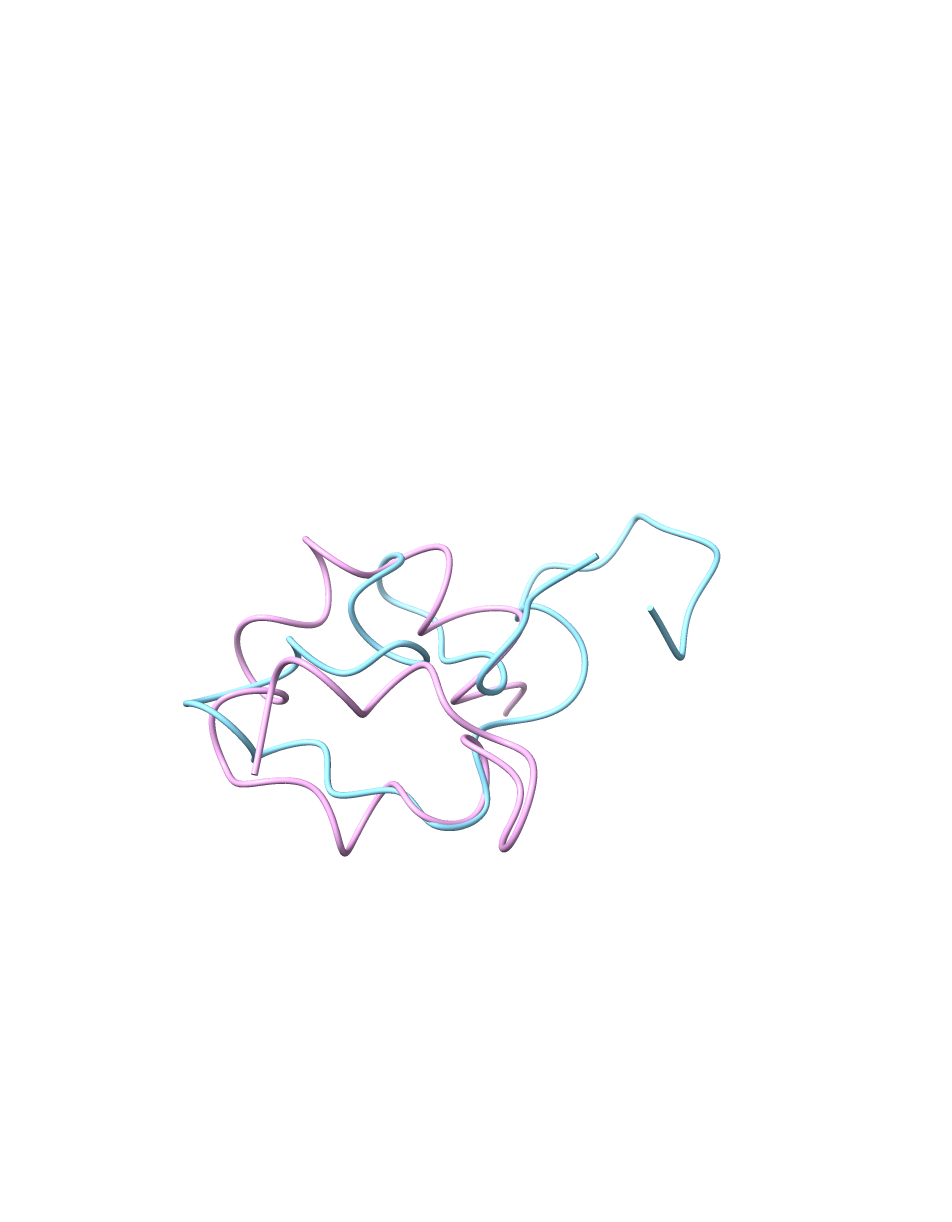
\includegraphics[width = 0.3\linewidth]{SET1.png}
        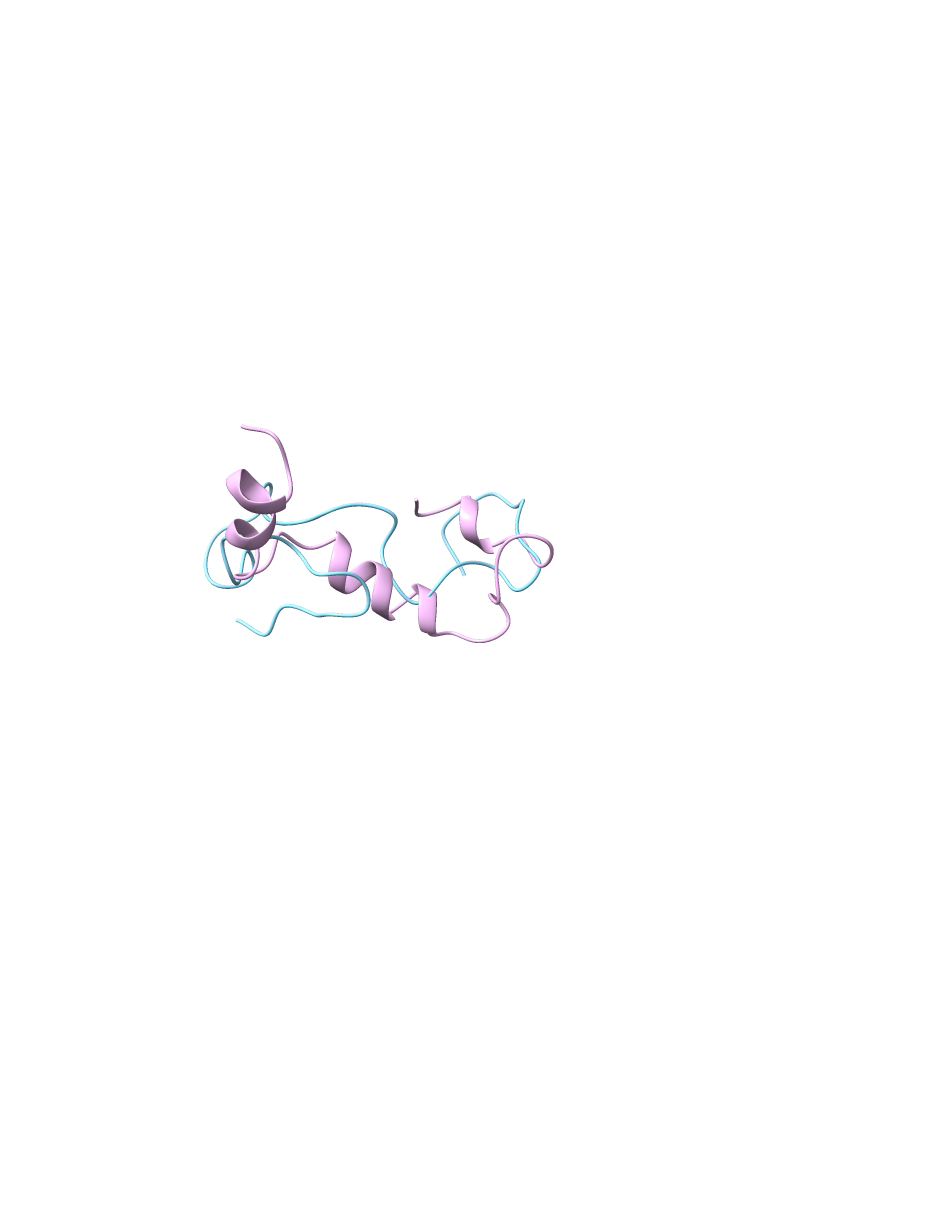
\includegraphics[width = 0.3\linewidth]{SET2.png}
        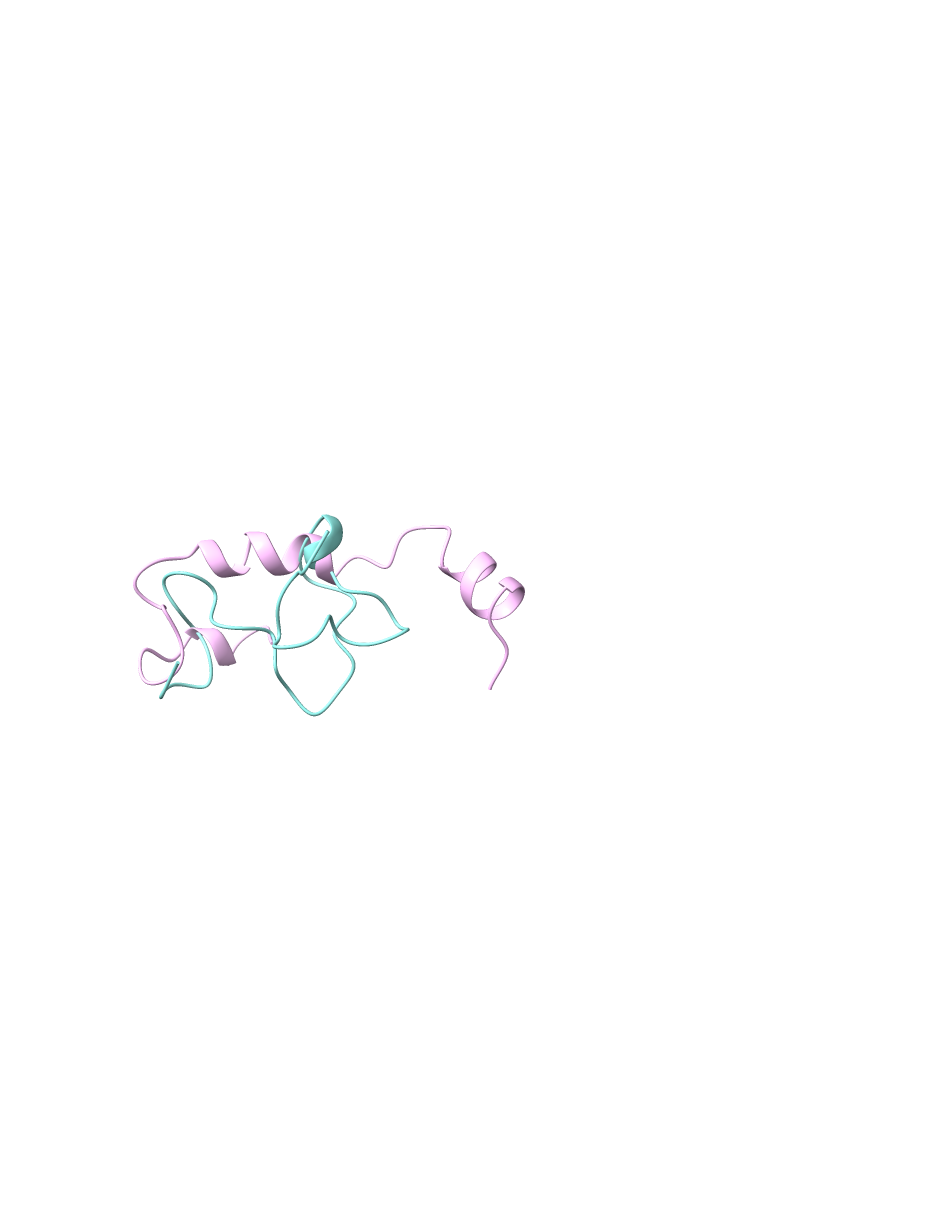
\includegraphics[width = 0.3\linewidth]{SET3.png}
 \caption Figure 3: {Overlays of the 3 sets of snapshots ranked from least to most energetic (Set 1, Set 2, Set 3)}\\


        The LVFFA pentapeptide segment was then extracted and capped with hydrogen atoms to avoid artificial charge artifacts. All geometric manipulations were performed on UCSF ChimeraX\cite{chimerax2018}, and capping was performed with RdKit\cite{rdkit}.\\
        \subsection{\textbf{Electronic Structure Problem Creation}}
 Electronic structure problems were created using PySCF\cite{pyscf2020} 2.7.0. The PySCF\cite{pyscf2020} driver was a dual-path driver function that integrates classical solvation effects using ddCOSMO ($\epsilon$=80.0). Each fragment was first modeled using PySCF\cite{pyscf2020}’s restricted Hartree-Fock (RHF) method, followed by ddCOSMO to simulate an aqueous environment. This structure captures key electrostatic effects relevant to biological environments. The molecular geometry, charge, and spin multiplicity were specified with Angstroms and STO-3G as the basis set. A shift of 0.2 was added to aid convergence. Selected HOMO-LUMO orbitals from were used to generate Gaussian cube files; prior energy identification runs were used to identify these orbitals(tables in supplement). To interface with the Quantum section, Qiskit-Nature\cite{qiskit2019}\cite{qiskit_nature2021}(0.7.2)’s PySCFDriver\cite{pyscf2020} was used to create an ElectronicStructureProblem object. This object will be mapped and used for the VQE\cite{peruzzo2014} run.

 \subsection{\textbf{Active Space Creation}}
To reduce computational overhead and focus on chemically relevant orbitals, I employed Qiskit\cite{qiskit2019} Nature’s ActiveSpaceTransformer to construct reduced Hamiltonians for variational quantum eigensolver (VQE\cite{peruzzo2014}) simulations.  The active space\cite{active_space} configuration explored was 4 orbitals/4 electrons (4o4e). These spaces were centered around the frontier orbitals, specifically the HOMO–LUMO region, with symmetric extensions of ±1 orbitals to capture near-degenerate excitations and charge-transfer character.
The active space\cite{active_space} was defined by selecting molecular orbitals relative to the canonical HOMO and LUMO indices obtained from PySCF\cite{pyscf2020}. This approach ensures that the most chemically and electronically significant orbitals are retained, while discarding deeply core and high-lying virtual orbitals that contribute minimally to correlation energy. The resulting second-quantized Hamiltonians were mapped to qubit operators using the Jordan-Wigner mapper. This strategy balances physical accuracy with quantum resource efficiency, enabling meaningful comparisons between Arctic and wild-type A$\beta$ fragments across conformational ensembles.\\
\subsection{\textbf{Quantum Simulation Protocol (Qiskit\cite{qiskit2019} 1.4.3)}}
Molecular integrals from each active space\cite{active_space} configuration were generated using PySCF\cite{pyscf2020} and down-folded into second-quantized Hamiltonians. These were mapped to qubit operators via the Jordan–Wigner transformation using Qiskit\cite{qiskit2019} -nature 0.7.2. Simulations targeted the LVFFA segment of Arctic and wild-type conformers, extracted from MD trajectories and capped with hydrogen atoms.
Two variational ansätze were employed:
\begin{itemize}
    \item Two local circuits with Ry and Rz rotation blocks and CZ entanglement (reps=2), optimized using the COBYLA(maxiter=200) classical optimizer. (Figure 4)
\end{itemize}
\begin{itemize}
    \item UCCSD (unitary coupled-cluster singles and doubles), initialized with Hartree–Fock reference states and optimized using COBYLA(maxiter=200). (Figure 5)
\end{itemize}

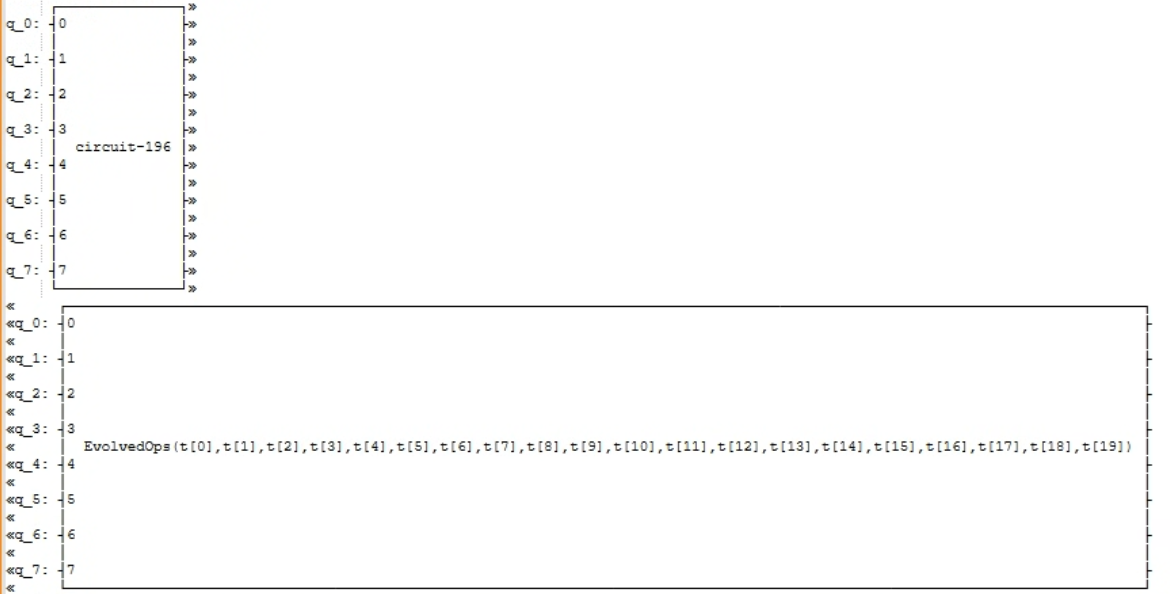
\includegraphics[width=0.95\linewidth]{UCCSD.png}
\caption\textbf{Figure 4: }{UCCSD Ansatz circuit diagram (Depth 196, 8 Qubits)}\\

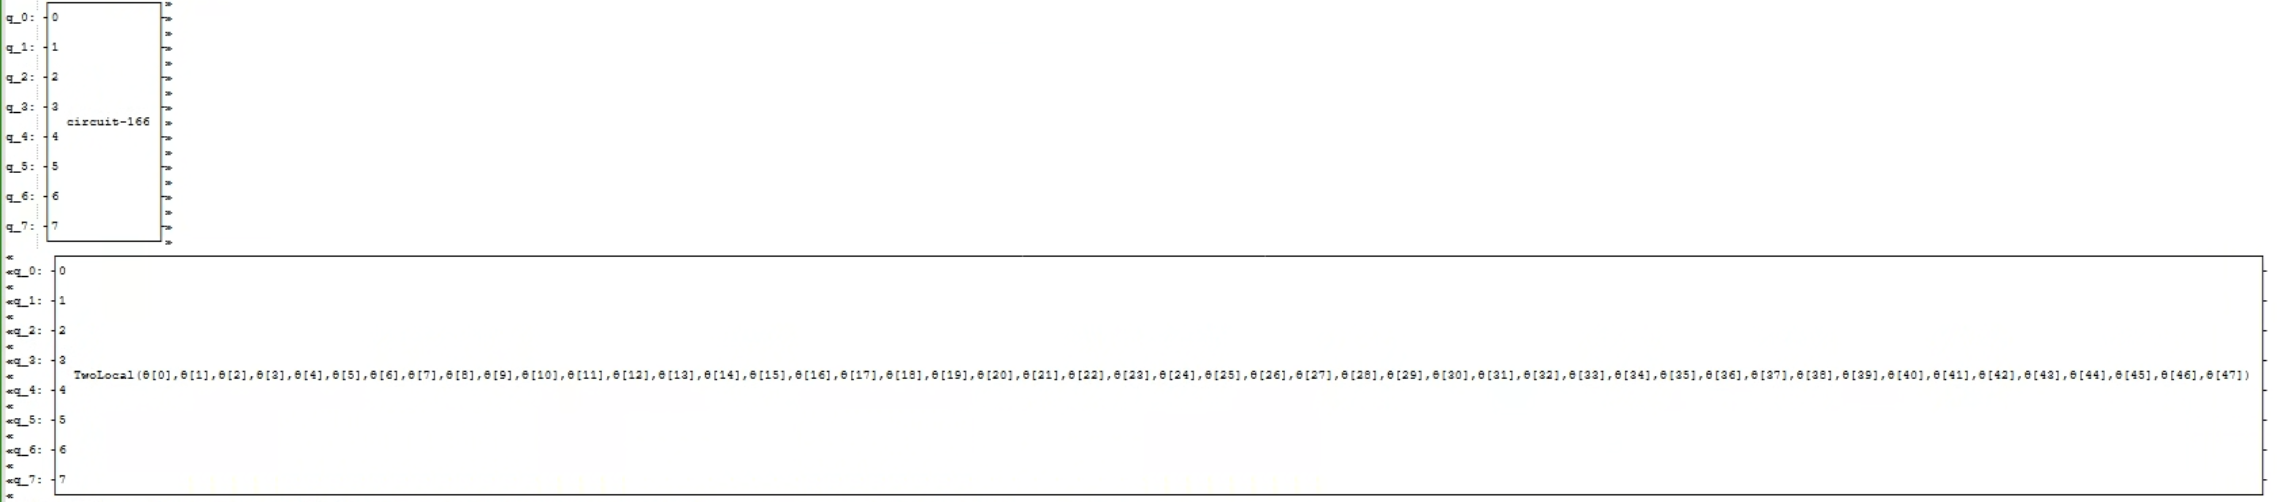
\includegraphics[width=0.95\linewidth]{TwoLocal.png}
\caption\textbf{Figure 5: }{TwoLocal Ansatz circuit diagram (Depth 166, 8 Qubits)}\\

All quantum simulations were performed on the Qiskit state vector simulator back end\cite{qiskit2019}. Total VQE\cite{peruzzo2014} energies were computed for Arctic and wild-type fragments across each active space\cite{active_space} configuration. The resulting energy gap ($\Delta$E) was used to quantify electronic stability differences and assess the impact of mutation on the energetics of the ground state.\\
\subsection{\textbf{Experimental Validation/Quantum Advantage}}

Classical force fields used in molecular dynamics lack explicit electronic structure, preventing direct calculation of mutation effects on electronic stability. While DFT could calculate these energies, VQE offers a systematically improvable approach that captures electron correlation exactly within the active space. Our results—showing conformation-dependent electronic stabilization—align with experimental aggregation data, demonstrating that quantum electronic structure calculations can reveal biophysically relevant mutation effects

\textbf{(Need to add citations)}
Experimental studies using thioflavin T fluorescence and kinetic modeling showed Arctic mutation increases the secondary nucleation rate by over 100-fold compared to wild-type. In cell culture, Arctic aggregates appear within 24 hours, while wild-type shows minimal aggregation. Our quantum calculations provide the electronic explanation: the E22G mutation creates conformation-dependent stabilization, making compact, aggregation-prone structures up to 0.05 Hartrees more stable. This electronic preference directly drives the mutation toward states that accelerate fibril surface nucleation - exactly matching the experimental 100-fold rate enhancement. The quantum calculations reveal why the mutation aggregates faster at the electron level.
        
		\section{Results}
        \subsection{\textbf{All-atom MD}}

To probe the structural landscape, all-atom MD for wild-type and Arctic Amyloid beta was performed. From the production trajectories, potential energy profiles were extracted using gmx\cite{gromacs2015} energy. Conformational Stability was assessed using the resulting XVG graphs with pronounced energy fluctuations, consistent with transient stabilization events. Rather than relying on a single snapshot, I extracted the top three lowest-energy conformers from each trajectory using gmx\cite{gromacs2015} trjconv -dump(Figure 6), ensuring coverage of the most populated basin. These conformers were capped with hydrogen atoms to yield chemically complete LVFFA fragments suitable for quantum analysis. Gmx\cite{gromacs2015} dssp and clustering (Figures 7 and 8) confirmed that the selected Arctic conformers were structurally compact and $\beta$-sheet–enriched, while wild-type conformers displayed greater backbone flexibility and coil-like features.\\\\
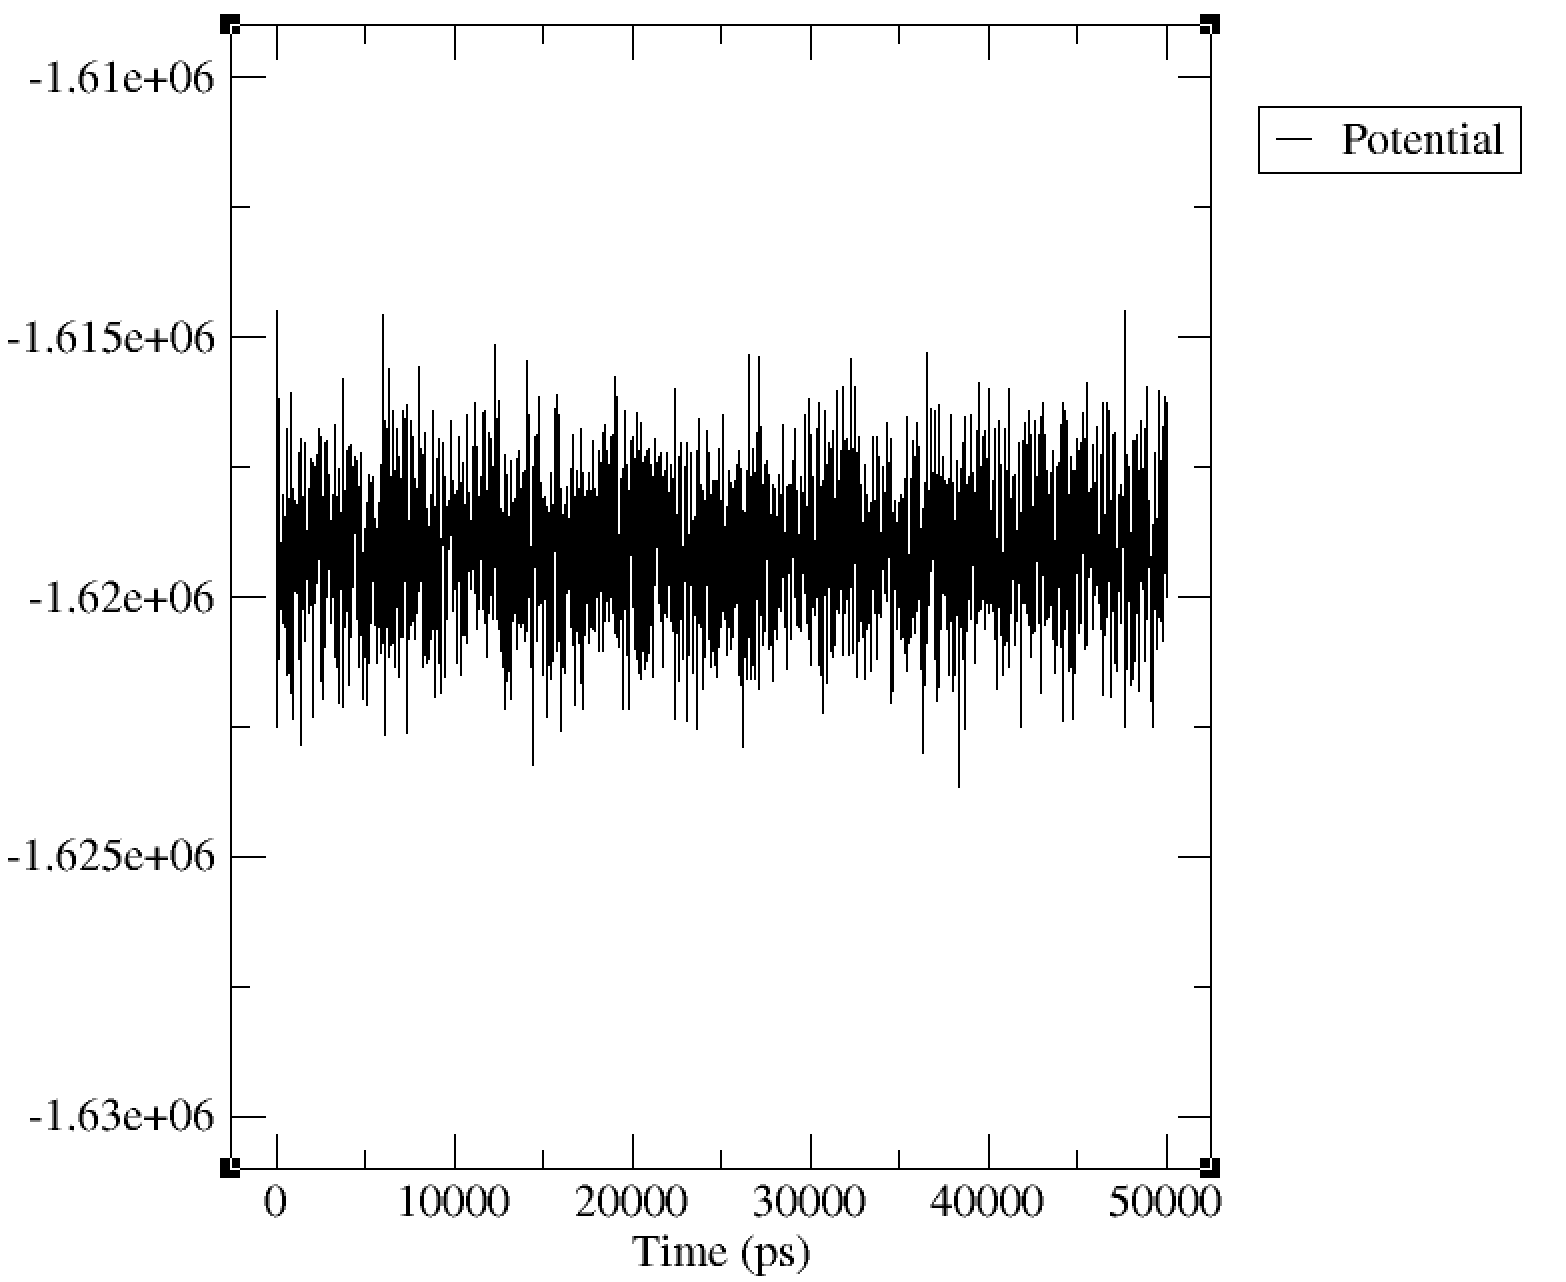
\includegraphics[width=0.48\linewidth]{AVPT.png}
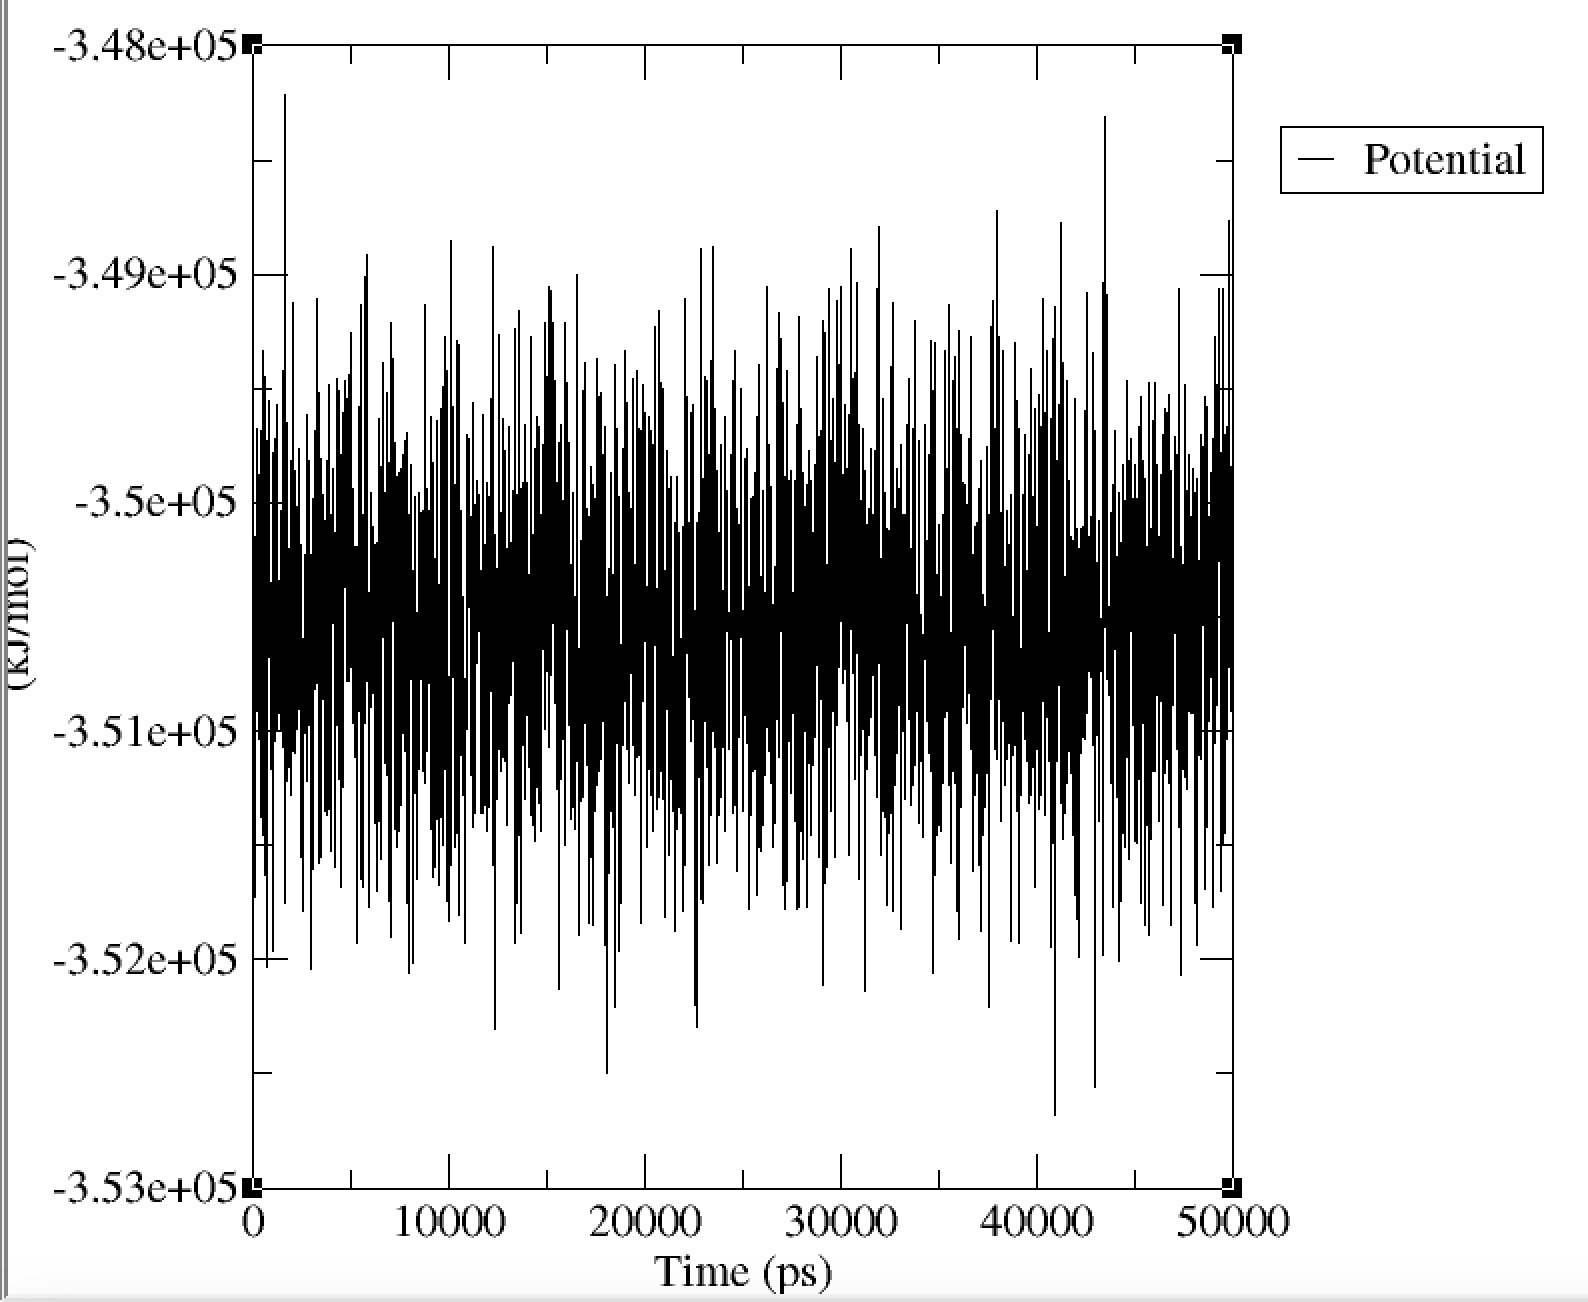
\includegraphics[width=0.48\linewidth]{WTPT.png}
\caption\textbf{Figure 6: }{Time evolution of the potential energy during molecular dynamics simulations of the amyloid-beta peptide. The graph displays the total potential energy(kJ/mol) as a function of simulation time for both wild-type and Arctic variants (E22G) (WT on right, Arctic on left)}\\
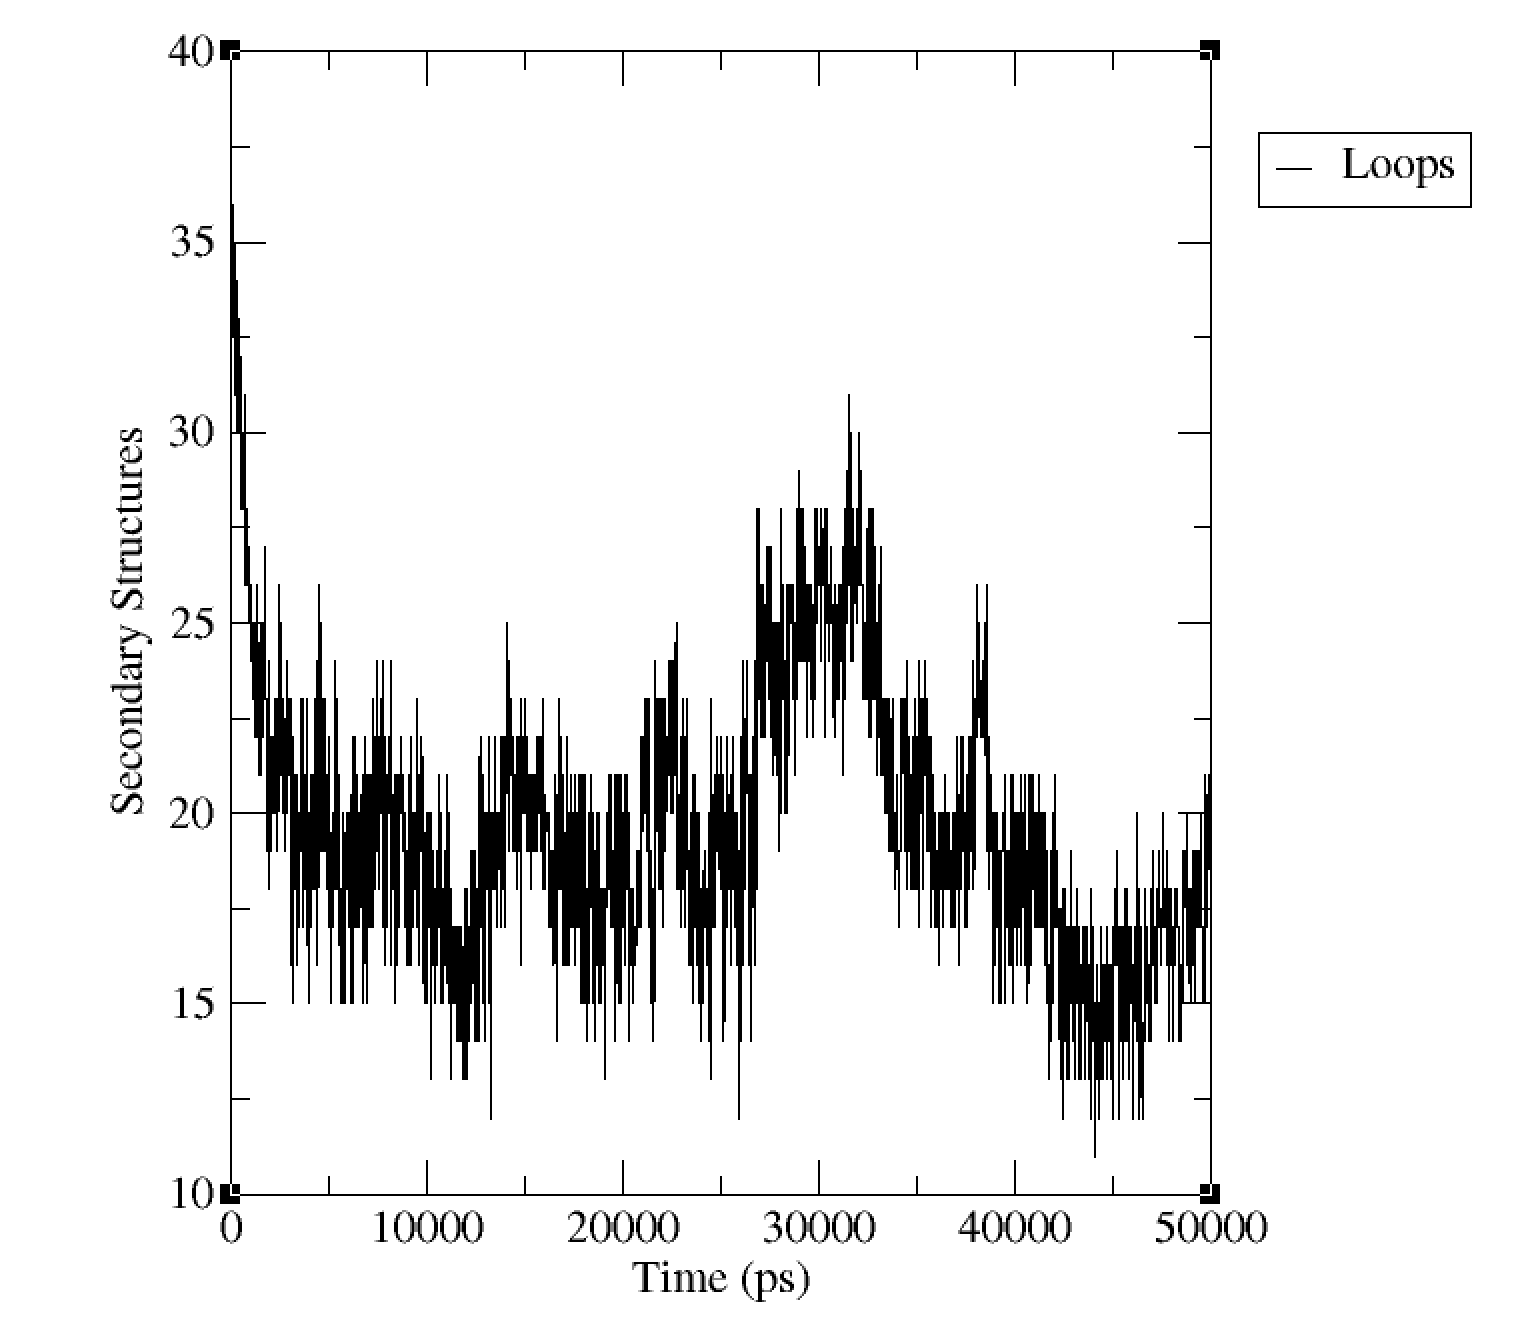
\includegraphics[width=0.48\linewidth]{SSA.png}
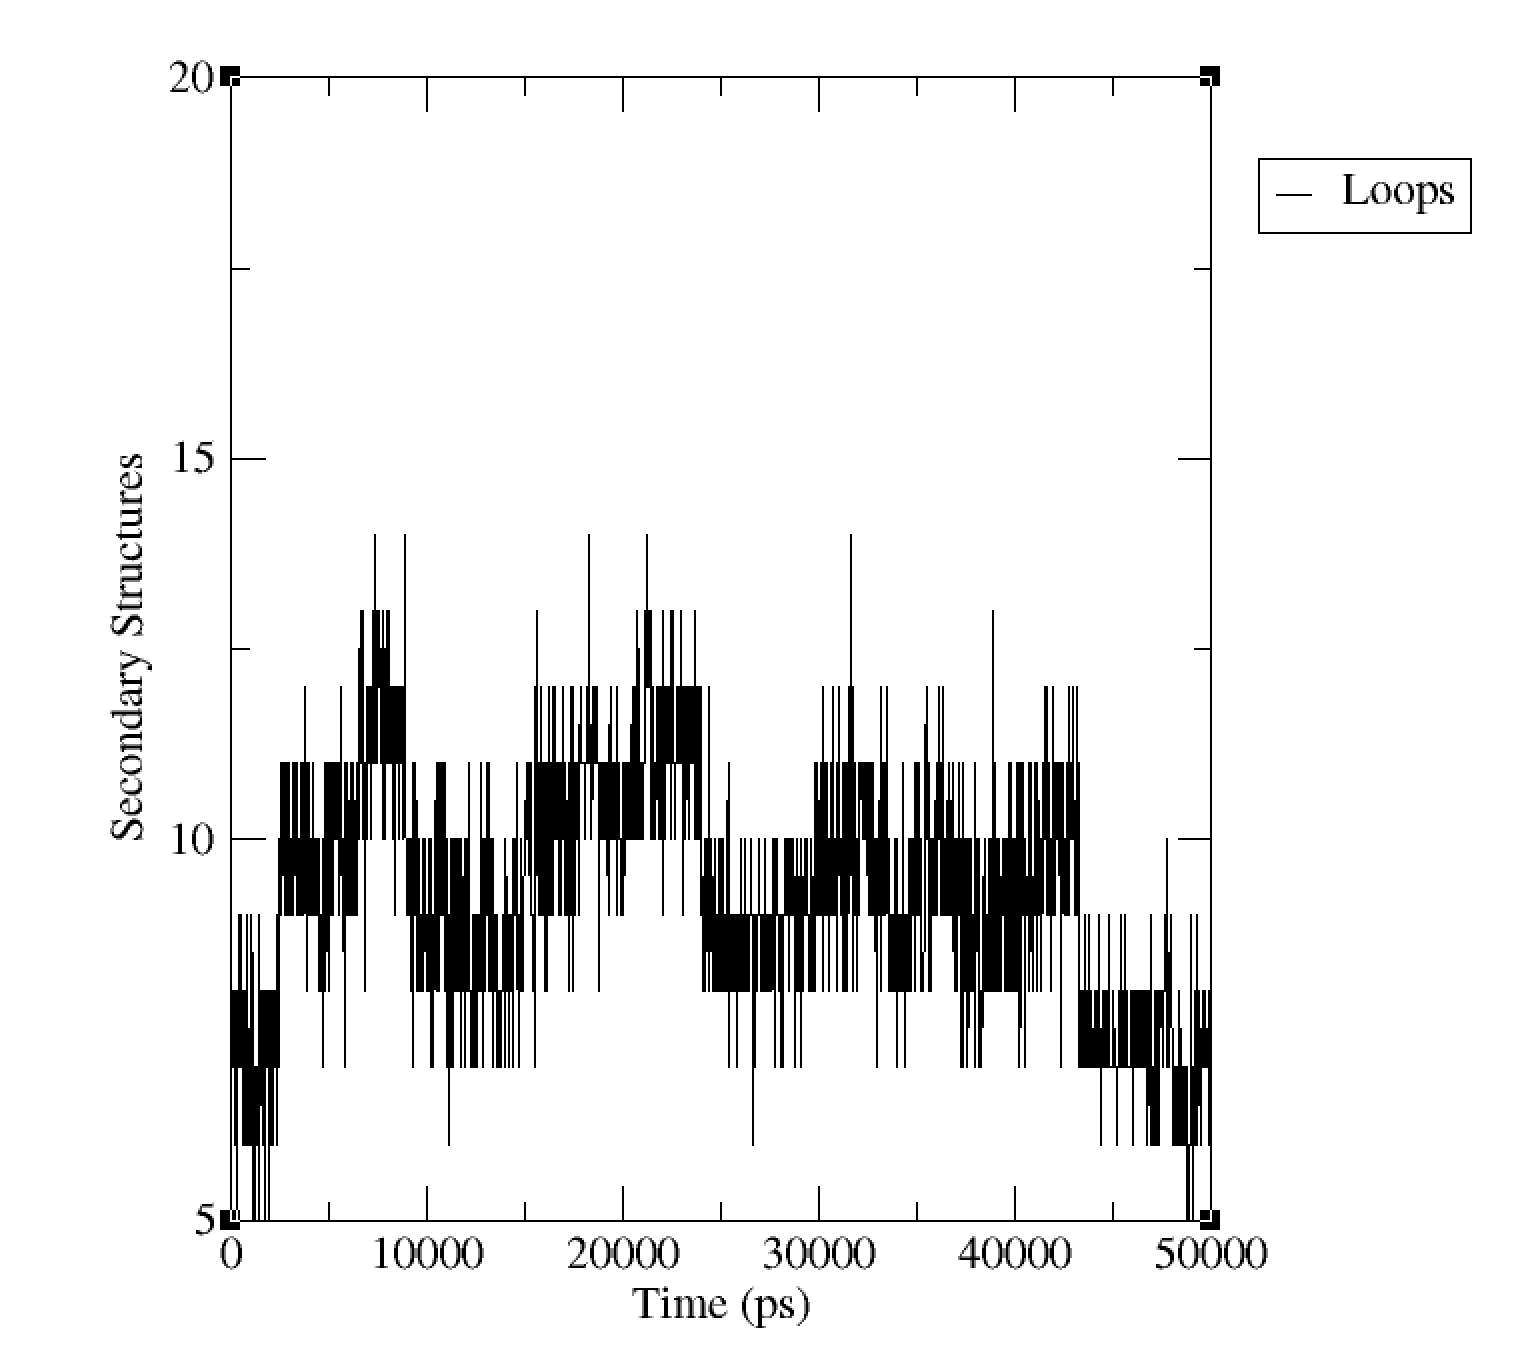
\includegraphics[width=0.48\linewidth]{SSWT.png}
\caption\textbf{Figure 7: }{Secondary structure assignment (DSSP) over the course of molecular dynamics simulations for wild-type and Arctic (E22G) amyloid-beta variants. (WT on right, Arctic on left)}\\
\includegraphics[width=0.48\linewidth]{arctic.png}
\includegraphics[width=0.48\linewidth]{wt.png}
\caption\textbf{Figure 8: }{Cluster population analysis of amyloid-beta peptide molecular dynamics trajectories. The bar plot shows the relative population of each conformational cluster identified from the whole production simulation, with clusters ranked by decreasing population. Peaks correspond to the most frequently sampled conformations. (WT on right, Arctic on left)}\\
\subsection{\textbf{Quantum Readiness and Fragment Stability}}

Each capped conformer was subjected to geometry optimization and orbital analysis via PySCF\cite{pyscf2020}. HOMO–LUMO gaps and orbital localization patterns were consistent across Arctic conformers, supporting their electronic stability. These fragments were then used for downstream DFT and VQE\cite{peruzzo2014} simulations, enabling ensemble-level comparison of electronic energies and mutation-induced stabilization.

\subsection{\textbf{Electronic Structure and Active Space Selection}}

Molecular orbital analysis of each representative snapshot revealed well-defined frontier orbitals localized predominantly on the LVFFA core. I selected a consistent active space\cite{active_space} spanning four spatial orbitals centered around the HOMO–LUMO pair to capture key electronic correlations. Orbital isosurface plots comparing Arctic and wild-type variants (Figure 9) illustrate subtle but meaningful changes in electronic density distribution induced by the E22G mutation, supporting the rationale for active space\cite{active_space} targeting.

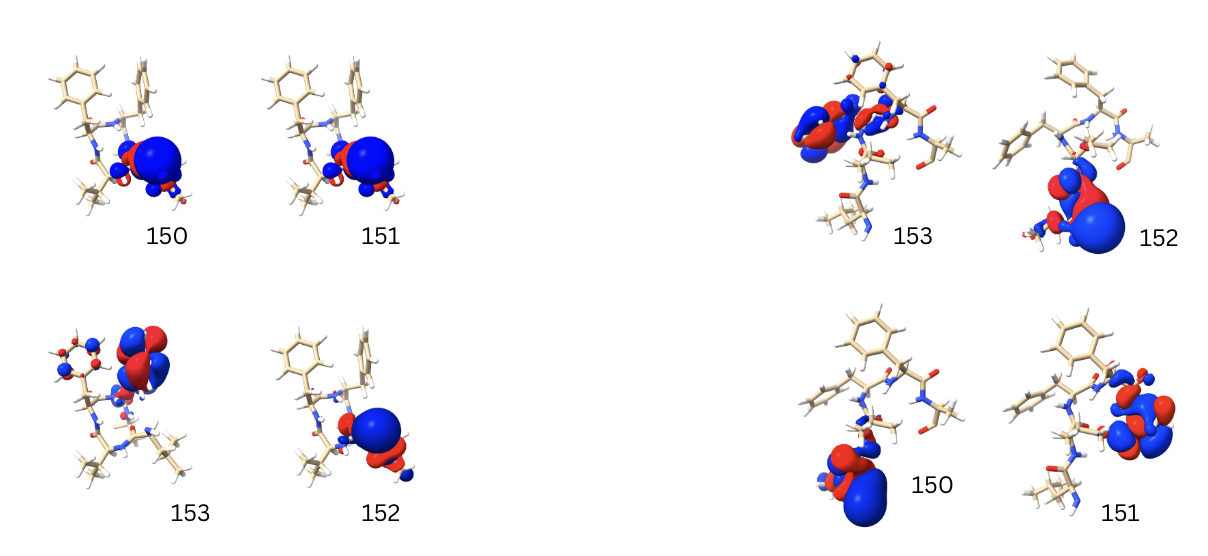
\includegraphics[width=0.95\linewidth]{SET1CUBE.png}
\begin{center}
Set 1
\end{center}
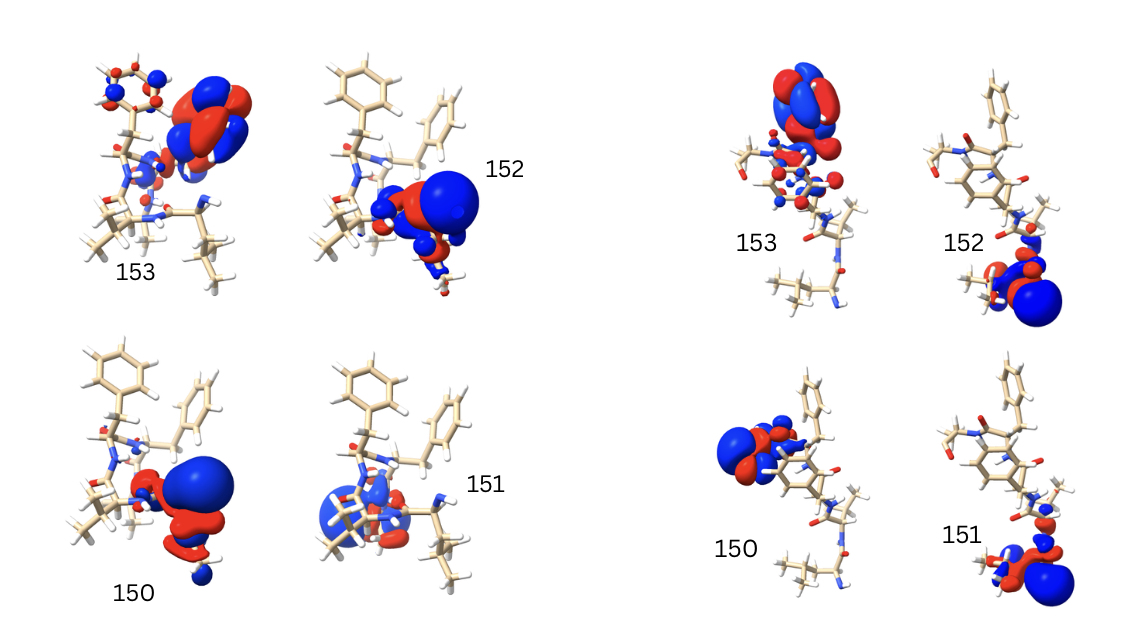
\includegraphics[width=0.95\linewidth]{SET2CUBE.png}
\begin{center}
Set 2
\end{center}
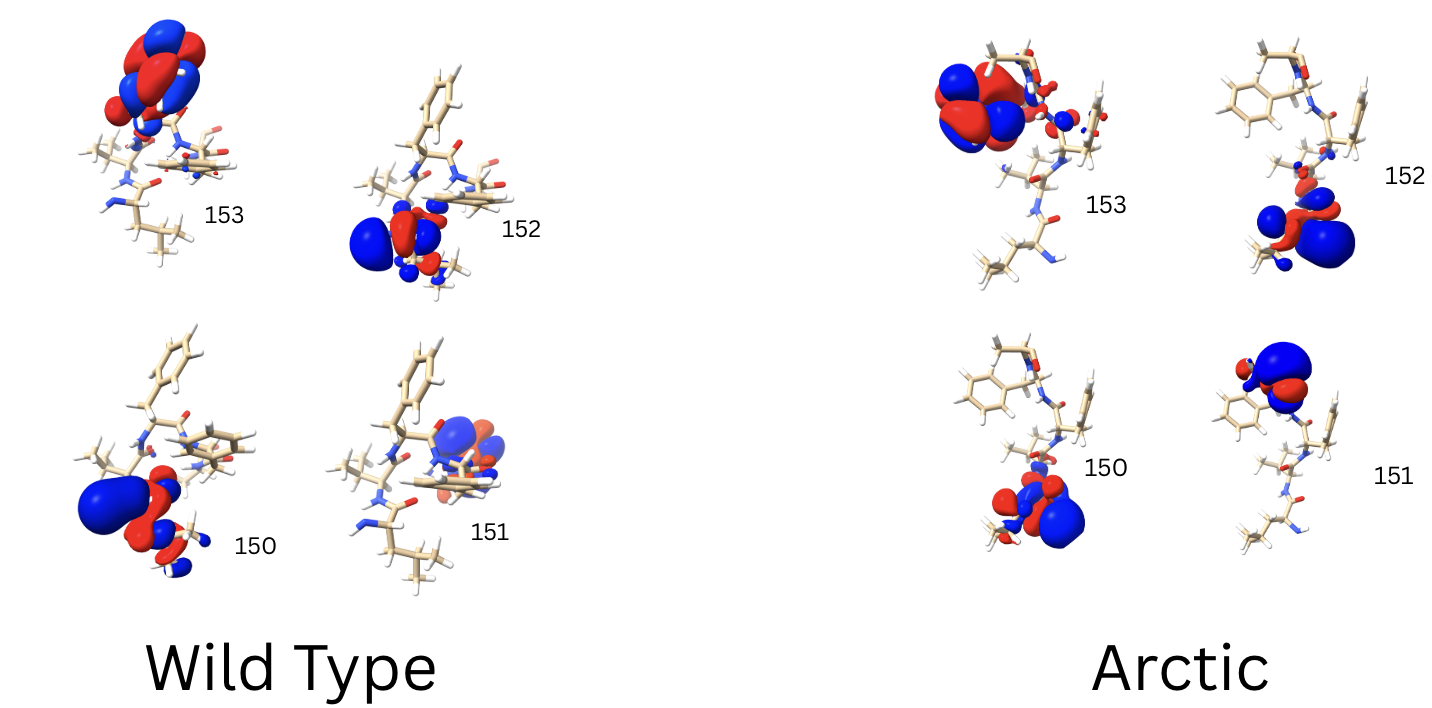
\includegraphics[width=0.95\linewidth]{SET3CUBE.png}
\begin{center}
Set 3
\end{center}
\caption\textbf{Figure 9: }{Visualization of HOMO-LUMO +/-1 Gaussian cube files depicting orbital isosurface amplitude from set 1. Generated by PySCF[11], visualized by ChimeraX[9], isovalue +/- 0.01 au, Red indicates the negative orbital surface, Blue indicates the positive orbital surface.}
        
\subsection{\textbf{Variational Quantum Eigensolver Convergence and Robustness}}

VQE\cite{peruzzo2014} calculations employing a TwoLocal ansatz with COBYLA optimization converged reliably across all three representative snapshots, as shown by energy convergence curves (Figures 10 and 11). The ansatz circuit depth and qubit count were sufficient to capture the essential correlation effects within the active space\cite{active_space}. Preliminary tests with alternative ansatzes, ie. UCCSD further confirms that the observed results are robust concerning the choice of quantum circuit architecture.\\
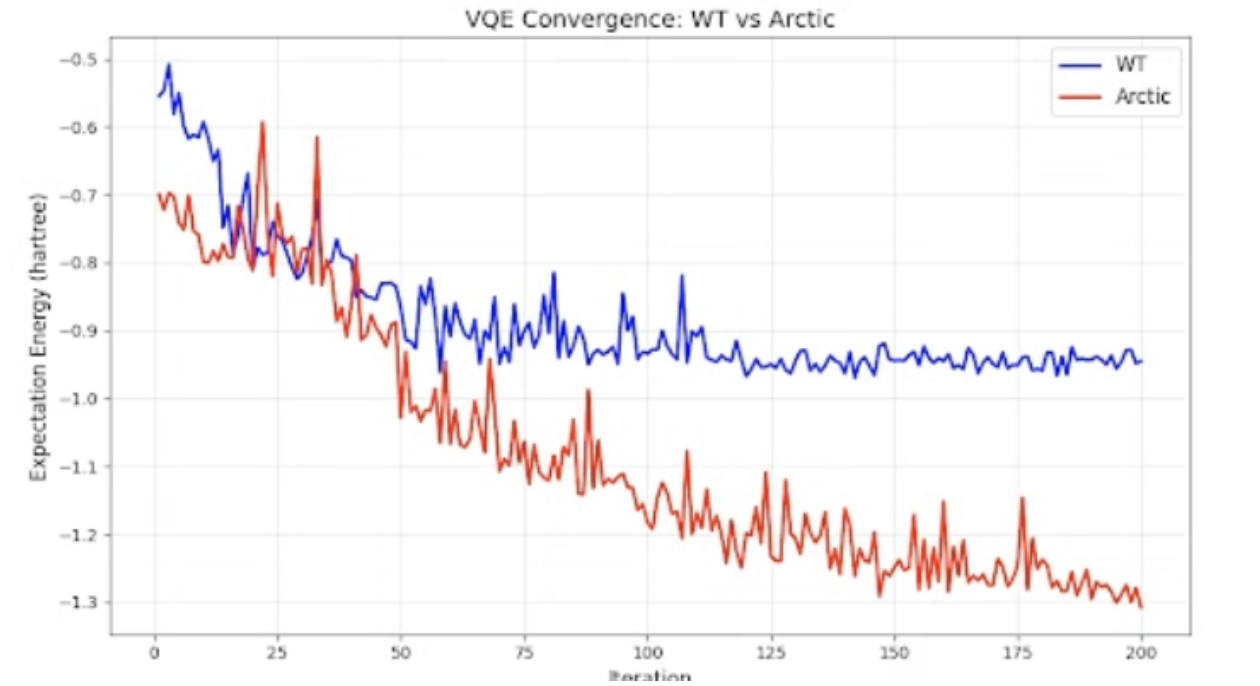
\includegraphics[width=0.95\linewidth]{SET1TLC.png}
\begin{center}
Set 1
\end{center}
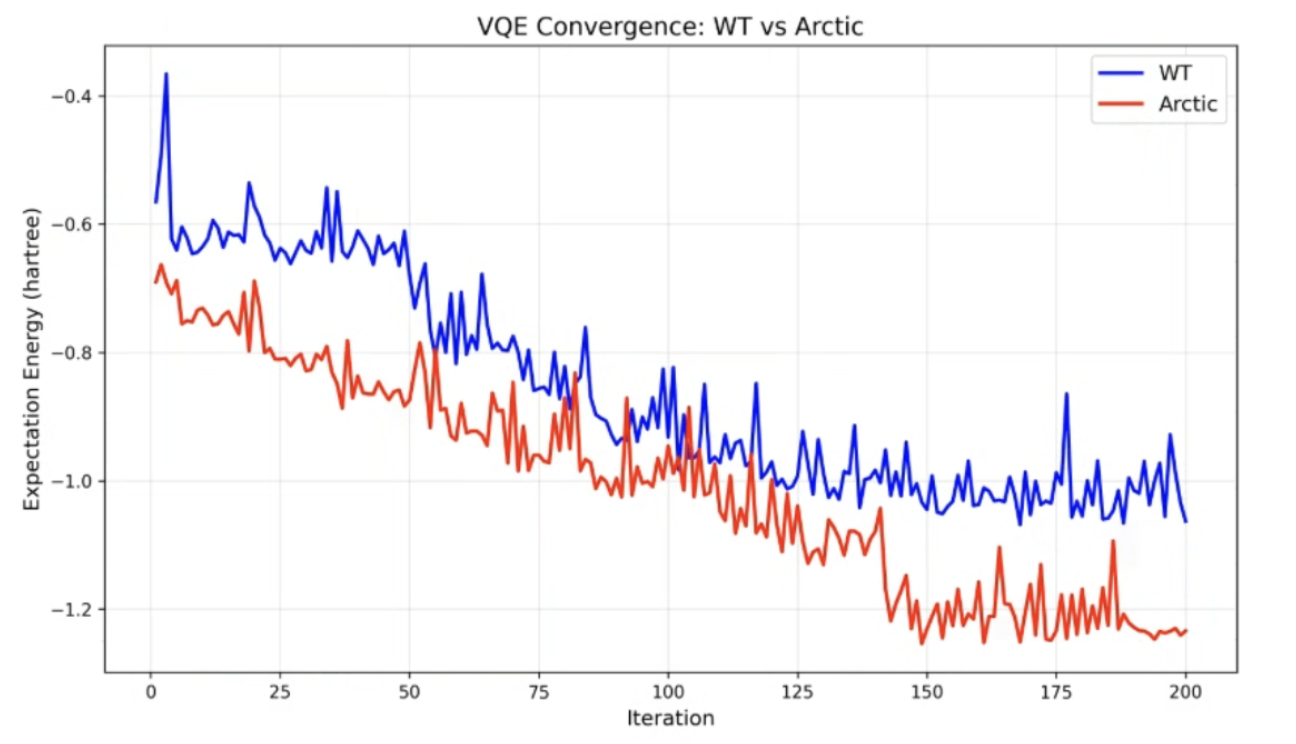
\includegraphics[width=0.95\linewidth]{SET2TLC.png}
\begin{center}
Set 2
\end{center}
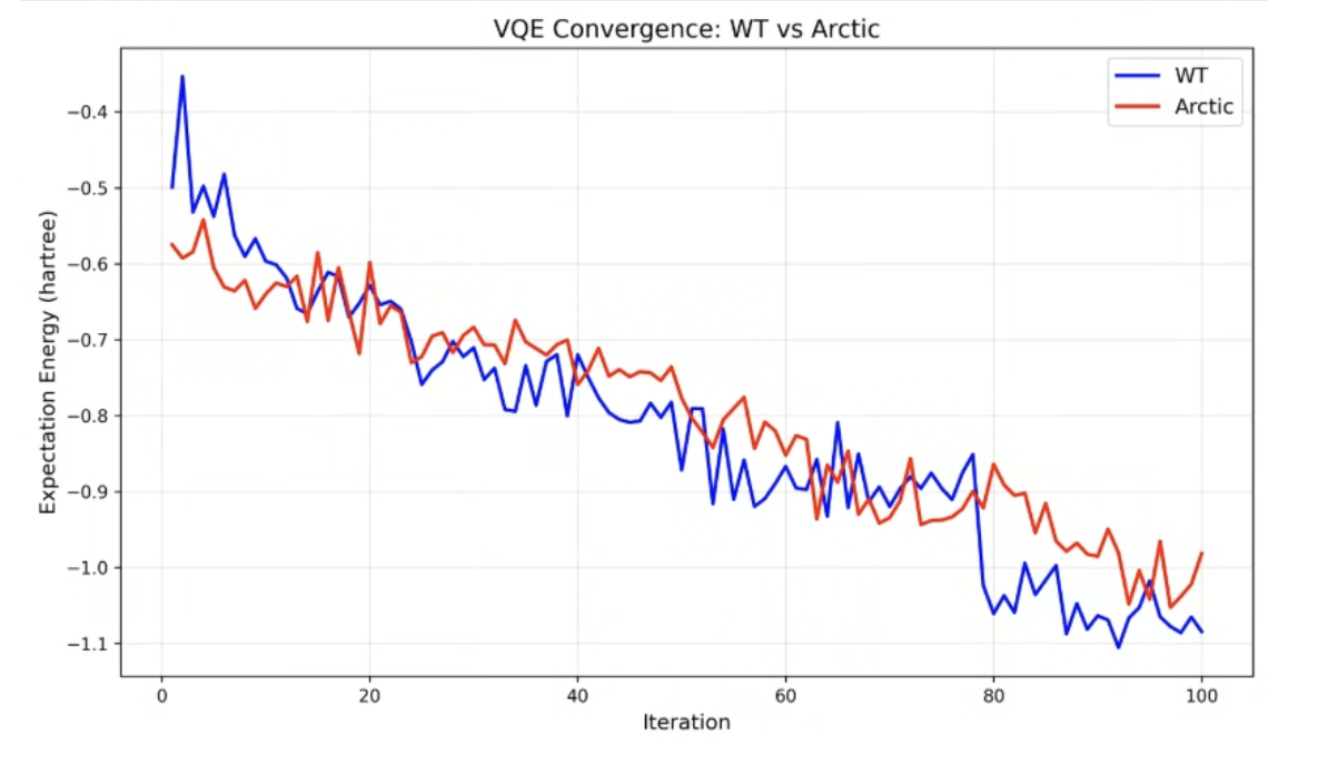
\includegraphics[width=0.95\linewidth]{SET3TLC.png}
\begin{center}
Set 3
\end{center}
\caption\textbf{Figure 10: }{VQE convergence plots for the TwoLocal Ansatz with COBYLA optimizer}\\

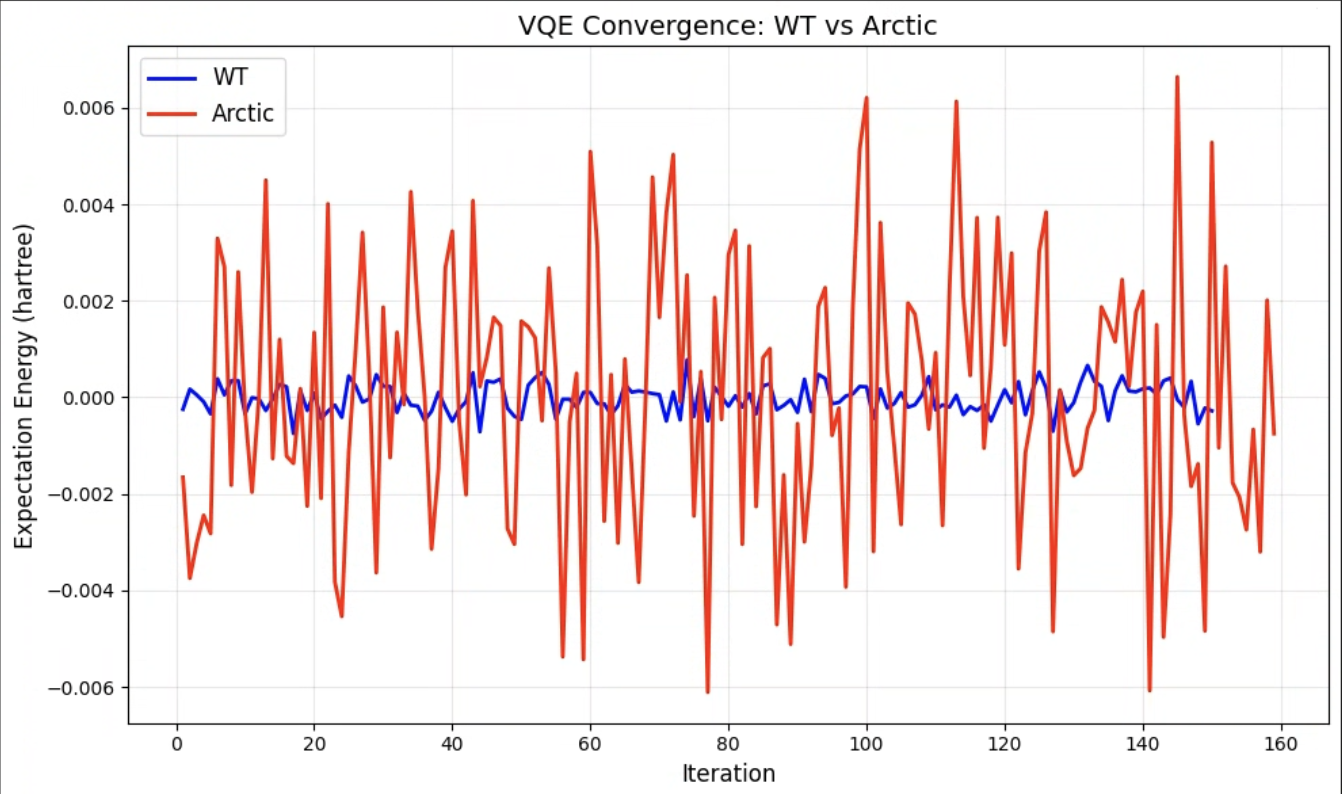
\includegraphics[width=0.95\linewidth]{set1ucc.png}
\begin{center}
Set 1
\end{center}
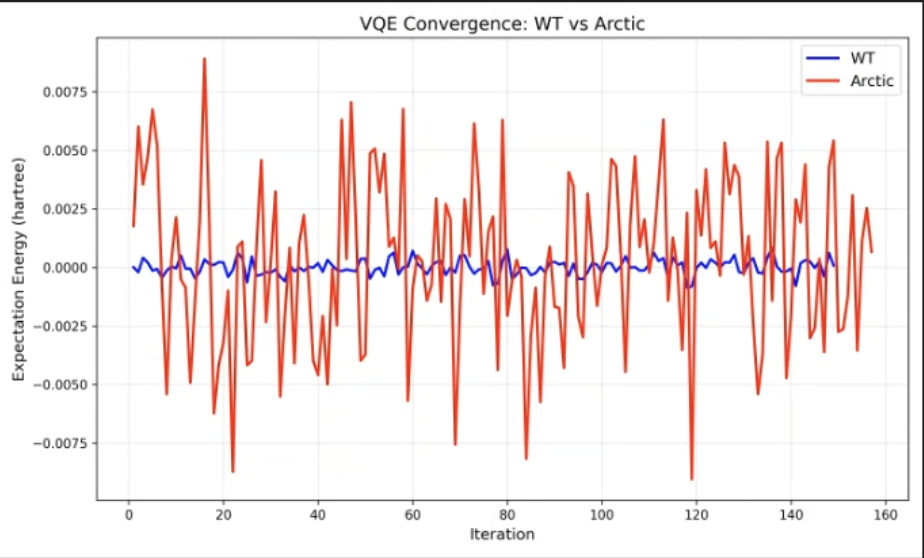
\includegraphics[width=0.95\linewidth]{set2ucc.png}
\begin{center}
Set 2
\end{center}
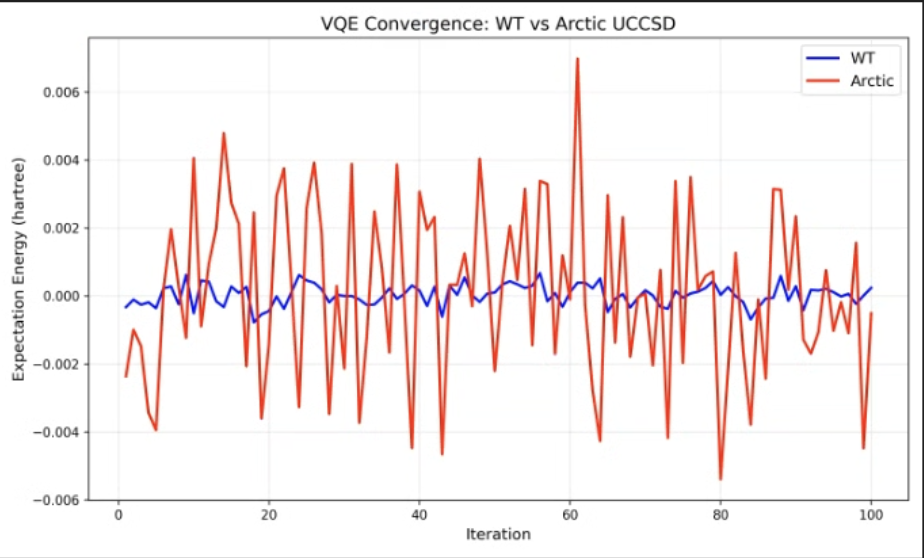
\includegraphics[width=0.95\linewidth]{set3ucc.png}
\begin{center}
Set 3
\end{center}
\caption\textbf{Figure 11: }{VQE\cite{peruzzo2014} convergence plots for the UCCSD Ansatz with COBYLA optimizer. The blue line (WT) demonstrates rapid and stable convergence to a low energy value. The red line (Arctic) also converges to a stable low-energy region, but its path is characterized by small, contained fluctuations with a total variation of less than 0.02. This contrast highlights the two distinct types of stability: ideal stability (WT) versus stochastic stability (Arctic).}\\


\begin{minipage}{\linewidth}
    \centering
    \scalebox{0.85}{ % shrink to 85% of column width
    \begin{tabular}{lccc}
        \hline
        \textbf{Final Energies TwoLocal} & \textbf{set 1} & \textbf{set 2} & \textbf{set 3} \\
        \hline
        WT: & -1805.442 & -1805.340 & -1805.479 \\
        Arctic: & -1805.608 & -1805.808 & -1805.401 \\
        $\Delta E$: & -0.161 & -0.338 & 0.077 \\
        \hline
    \end{tabular}}
    \caption\textbf{Table 1: }{Mean Final Energies for Different Sets TwoLocal}
    \label{tab:final_energies_twolocal}
\end{minipage}

\vspace{5mm} % optional spacing
\begin{minipage}{\linewidth}
    \centering
    \scalebox{0.85}{ % shrink to 85% of column width
    \begin{tabular}{lccc}
        \hline
        \textbf{Final Energies UCCSD} & \textbf{set 1} & \textbf{set 2} & \textbf{set 3} \\
        \hline
        WT: & -1804.375 & -1804.375 & -1804.335 \\
        Arctic: & -1804.355 & -1804.383 & -1804.383 \\
        $\Delta E$: & 0.0198 & -0.0086 & -0.0486 \\
        \hline
    \end{tabular}}
    \caption\textbf{Table 2: }{Mean Final Energies for Different Sets UCCSD}
\end{minipage}\\

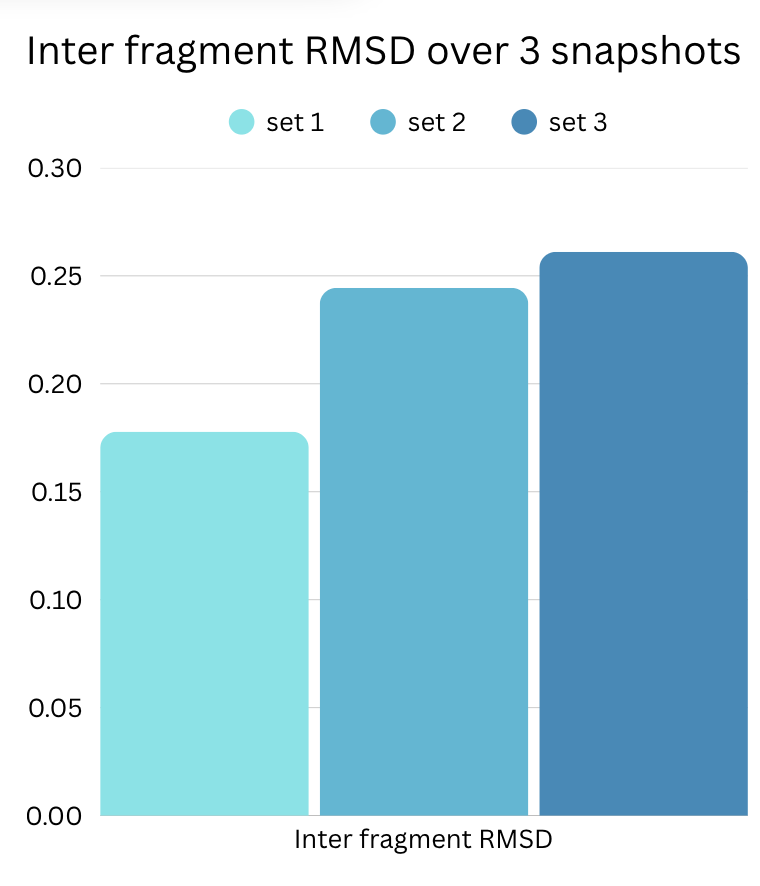
\includegraphics[width=0.95\linewidth]{IFRMSD.png}
\caption\textbf{Figure 12: }{Inter-fragment RMSD for each snapshot}



		\section{Discussion}
         Our results from this novel classical-quantum methodology yield a reproducible and translatable process that depicts the electronic and structural levels differences of wild-type and Arctic $\beta$-amyloid. In particular, the stabilization of the Arctic variant observed in the quantum simulations is consistent with its experimentally known increased fibrillation propensity and accelerated plaque formation. These results suggest that in this case subtle orbital energy shifts, specifically differences in the HOMO-LUMO gap, may be the basis for the altered aggregation kinetics observed in familial Alzheimer’s disease mutations.

Benchmarking against validated ORCA\cite{orca2020} B3LYP calculations for representative structures confirmed that VQE\cite{peruzzo2014} with a TwoLocal ansatz can perform accurate correlation effects, outperforming RHF and other heuristic approaches over trajectory snapshots. This demonstrates that our hybrid-classical quantum methodology is not limited by the noise of ansatzes and/or expressability challenges often cited in quantum computing literature. Moreover, by limiting orbital treatment to an active space\cite{active_space} by using the results of informed MD simulations, the run time was cut by orders of magnitude, which classical algorithms cannot accomplish.

Methodologically, this represents the first full integration of fully atomistic MD simulations with quantum electronic structure treatment on biologically relevant peptide fragments. While QM/MM simulations are well-established in the field of quantum chemistry, expanding the high-level region into a quantum computing paradigm can lead to deeper electronic insights in such biomolecular environments. Importantly, this methodology is hardware-agnostic and can be adapted for near-term quantum devices, enabling incremental improvements in accuracy as qubit counts and fidelities increase.

From a biomedical perspective, these findings motivate the exploration of mutation-specific electronic fingerprints in amyloidogenic peptides. If such quantum descriptors can be linked to aggregation rates or binding affinities, they could serve as computational biomarkers for early-stage therapeutic screening. From a computational science perspective, this study underscores the potential for variational quantum algorithms to tackle correlated electronic problems in realistic biological contexts, a domain traditionally out of reach for exact quantum chemistry at scale.

The VQE convergence plots(Figures 10 and 11) over the two ansatzes highlight the importance of ansatz selection in VQE runs. Based on the results extracted from the VQEs, the UCCSD ansatz's output would be a more accurate representation of the electronic level differences despite the chaotic convergence plots. This is because UCCSD's $\Delta$E alignment more closely matches the B3LYP output, and also because the UCCSD convergence output reflects the differences in 'types' of electronic stability that the Arctic and Wild Type Amyloid-Beta display. The ideal stability of the wild type and the stochastic stability of the Arctic type. The visible fluctuations, while contained within a very narrow total less than 0.02, are not a sign of failure, but rather a sign of a stochastic search method. This offers a powerful illustration of the complexity of quantum chemistry. 

Future work will focus on extending this methodology to explicit solvent environments, as well as testing alternative ansätze. As quantum hardware matures, our approach could scale to full-length $\beta$-amyloid peptides and beyond, paving the way for quantum-accelerated biophysics.


\section{Conclusions}\label{sec4}

In summary, our hybrid molecular dynamics - VQE\cite{peruzzo2014} framework establishes a transferable pathway to probe the electronic structure of biomolecular fragments at a level of accuracy traditionally restricted to prohibitively expensive correlation methods. By coupling atomistic sampling with quantum electronic structure treatment, electronic descriptors and stability trends are accessed that are inaccessible to conventional QM/MM partitioning. The approach is readily adaptable to other peptides and molecular systems of comparable scale, providing a generalizable tool for exploring correlation-driven phenomena in biologically relevant contexts. As quantum hardware advances, this methodology offers a route toward routine quantum-accelerated characterization of complex molecular systems.

\end{multicols}
\clearpage
\bibliographystyle{num}
\bibliography{sn-bibliography}
			

	
	\vspace{3cm}
	My github repo for this project:\\
	
	\url{https://github.com/kpis-him/qc_proj}
	
	
\end{document}